% !TEX TS-program = pdflatex
% !TEX encoding = UTF-8 Unicode

% This is a simple template for a LaTeX document using the "article" class.
% See "book", "report", "letter" for other types of document.
\PassOptionsToPackage{table}{xcolor}
\documentclass[12pt]{report} % use larger type; default would be 10pt

\usepackage[utf8]{inputenc} % set input encoding (not needed with XeLaTeX) 
\usepackage[finnish]{babel}
\usepackage[acronym,toc]{glossaries}


%%% Examples of Article customizations
% These packages are optional, depending whether you want the features they provide.
% See the LaTeX Companion or other references for full information.
\parindent0pt  \parskip10pt             % make block paragraphs

%%% PAGE DIMENSIONS
\usepackage{geometry} % to change the page dimensions
\geometry{a4paper} % or letterpaper (US) or a5paper or....
% \geometry{margin=2in} % for example, change the margins to 2 inches all round
% \geometry{landscape} % set up the page for landscape
% read geometry.pdf for detailed page layout information

\usepackage{graphicx} % support the \includegraphics command and options

% \usepackage[parfill]{parskip} % Activate to begin paragraphs with an empty line rather than an indent

%%% PACKAGES
\usepackage{booktabs} % for much better looking tables
\usepackage{array} % for better arrays (eg matrices) in maths
\usepackage{paralist} % very flexible & customisable lists (eg. enumerate/itemize, etc.)
\usepackage{verbatim} % adds environment for commenting out blocks of text & for better verbatim
\usepackage{subfig} % make it possible to include more than one captioned figure/table in a single float
\usepackage{float}
% These packages are all incorporated in the memoir class to one degree or another...

% Custom colors for eg. links
\usepackage{xcolor}
\definecolor{airforceblue}{rgb}{0.36, 0.54, 0.66}
\definecolor{coolblack}{rgb}{0.0, 0.18, 0.39}

%%% Make toc links clickable and hyperlinks available
\usepackage{hyperref}
\hypersetup{
    colorlinks,
    linktoc=all,
    citecolor=black,
    filecolor=black,
    linkcolor=coolblack,
    urlcolor=black
}

%%% HEADERS & FOOTERS
\usepackage{fancyhdr} % This should be set AFTER setting up the page geometry
\pagestyle{fancy} % options: empty , plain , fancy
%\renewcommand{\headrulewidth}{0pt} % customise the layout...


% Lorem ipsum dolor depsum...
\usepackage{lipsum}

%%% SECTION TITLE APPEARANCE
%\usepackage{sectsty}
%\allsectionsfont{\sffamily\mdseries\upshape} % (See the fntguide.pdf for font help)
% (This matches ConTeXt defaults)


%%% TABLE STYLING
%\setlength{\arrayrulewidth}{1mm}
\setlength{\tabcolsep}{10pt}
\renewcommand{\arraystretch}{1.5}
   
%%% ToC (table of contents) APPEARANCE
\usepackage[nottoc,notlof,notlot]{tocbibind} % Put the bibliography in the ToC
\usepackage[titles,subfigure]{tocloft} % Alter the style of the Table of Contents
\renewcommand{\cftsecfont}{\rmfamily\mdseries\upshape}
\renewcommand{\cftsecpagefont}{\rmfamily\mdseries\upshape} % No bold!

%\renewcommand{\chaptername}{Kappale}
%renewcommand{\contentsname}{Sisällys}
%\renewcommand{\tablename}{Taulukko}
%\renewcommand{\figurename}{Kuva}


%%% END Article customizations
\graphicspath{ {./images/} }

%%% The "real" document content comes below...

\title{TIE-02301 Johdatus ohjelmointiin: Harjoitustyö 1}
\author{Kujanen J., Palonen J., Siiranen S \& Werner, V}

%%% HEADERS & FOOTERS
\lhead{TIE-02301 Johdatus ohjelmointiin: Harjoitustyö 1}\chead{}\rhead{Versio \currentversion}
\lfoot{fffilename.pdf

%%% IMPORTANT! This file should ONLY contain the name on the output pdf on the first line.
}\cfoot{\thepage}\rfoot{\textit{Muokattu \today}}


%%% Make toc start at 0 instead of 1 by setting this to -1
\pagenumbering{roman}                   % roman page number for toc and versions
\setcounter{chapter}{0}

% Lyhenteet mukaan 
\setglossarystyle{altlist}
%
%%% LYHENTEET JA MÄÄRITELMÄT (+ käännökset?)
%
% Tässä tiedostossa määritellään tekstissä kätetyt lyhenteet
%
% LaTeX rakentaa näistä automaattisesti sivun, jossa esitellään kaikki
% dokumentissa esiintyvät lyhenteet (akronyymit). Valmiissa pdf:ssä
% jokainen lyhenne on myös linkki sen määritelmään, eli linkkiä 
% klikkaamalla pääsee suoraan sen määritelmään. 

\makeglossaries

    \newacronym{gdpr}{GDPR}{General Data Protection Regulation}
    \newacronym{crm}{CRM}{Customer Relationship Management}
    \newacronym{erp}{ERP}{Enterprise Resource Planning}
    \newacronym{ups}{UPS}{Uninterupted Powersource}


    \newglossaryentry{gdprg}
    {
    name={General Data Protection Regulation (GDPR)},
	description={General Data Protection Regulation on Euroopan unionin asettama direktiivi tietosuojakäytännöistä},
	first={General Data Protection Regulation (GDPR)},
	text={GDPR}
    }
    \glsadd{gdprg}

    \newglossaryentry{crmg}
    {
	name={Customer Relationship Management (CRM)},
	description={Customer Relationship Management eli asiakkuudenhallintajärjestelmä},
	first={Customer Relationship Management (CRM)},
	text={CRM}
    }
    \glsadd{crmg}

    \newglossaryentry{erpg}
    {
    name={Enterprise Resource Planning (ERP)},
    description={toiminnanohjausjärjestelmä on yrityksen tietojärjestelmä, joka integroi eri toimintoja, esimerkiksi tuotantoa, jakelua, varastonhallintaa, laskutusta ja kirjanpitoa}
    first={Enterprise Resource Planning (ERP)}
    text={ERP}
    }
    \glsadd{erpg}

    \newglossaryentry{upsg}
    {
    name={Uninterupted Power Supply (UPS)}
    description={järjestelmä, joka takaa tasaisen virransyötön, vaikka järjestelmän ulkopuolinen virransyöttö katkeaisi tai virransyötössä ilmenee joku muu häiriö.}
    first={Uninterupted Power Supply (UPS)}
    text={UPS}
    }
    \glsadd{upsg}

    \newglossaryentry{kayttajag}
    {
    name={Käyttäjä},
    description={Henkilö tai taho, joka jollain tavalla hyödyntää järjestelmää}
    }
    \glsadd{kayttajag}

    \newglossaryentry{ulkoinenkayttajag}
    {
    name={Ulkoinen käyttäjä},
    description={Yksityis- tai yritysasiakas}
    }
    \glsadd{ulkoinenkayttajag}

    \newglossaryentry{sisainenkayttajag}
    {
    name={Sisäinen käyttäjäg},
    description={Kaikki konsernin sisällä toimivat tahot, jotka hyödyntävät järjestelmää. (esim. myynti- ja markkinointiosasto)}
    }
    \glsadd{sisainenkayttajag}

    \newglossaryentry{paakayttajag}
    {
    name={Pääkäyttäjä}
    description={Henkilö, joka käyttää järjestelmää säännöllisesti ja vastaa sen sisällön tuottamisesta}
    }
    \glsadd{paakayttajag}

    \newglossaryentry{tietokantag}
    {
    name={Tietokanta}
    description={tietojen keräämiseen ja järjestämiseen käytettävä työkalu, johon voidaan tallentaa esimerkiksi henkilöihin, tuotteisiin tai tilauksiin liittyviä tietoja}
    }
    \glsadd{tietokantag}

    \newglossaryentry{reduntantg}
    {
    name={reduntant}
    description={varmistettu (kahdennettu) linkki, joka toimii varana, jos ensisijainen järjestelmä kaatuu}
    }
    \glsadd{reduntantg}

    \newglossaryentry{virtualg}
    {
    name={virtualisointi}
    description={leikitään että resurssit on jotain muuta kun ne oikeesti on}
    }




\begin{document}


    % Custom Titlepage, you may use \maketitle as well to use embedded values

    \begin{titlepage}
        \centering
        %\includegraphics[width=0.15\textwidth]{example-image-1x1}\par\vspace{1cm}
        {\scshape\LARGE Tampereen Teknillinen Yliopisto \par}
        \vspace{1cm}
        {\scshape\Large TIE-02301 Johdatus ohjelmointiin\par}
        \vspace{2.5cm}
        {\huge\bfseries Harjoitustyö 1 \par}
        %{\huge\bfseries Megantti konsernin asiakastietojärjestelmä\par}
        \vspace{4cm}
        {\Large\itshape Jussi \textsc{Kujanen}, \textit{273161}\par}
	    {\quad \textit{jussi.kujanen@tuni.fi \newline} }
        {\Large\itshape Joonas\textsc{Palonen}, \textit{272784}\par}
	    { \quad \textit{joonas.palonen@tuni.fi \newline} }
        {\Large\itshape Santeri \textsc{Siiranen}, \textit{284281}\par}
	    { \quad \textit{santeri.siiranen@tuni.fi \newline} }
        {\Large\itshape Ville \textsc{Werner}, \textit{273022}\par}
	    { \quad \quad \textit{ville.werner@tuni.fi \newline} }
        
        \vfill
%        Suorituspaikka: \textsc{???}
    
        \vfill
    
    % Bottom of the page
        {\large \today \par}
    \end{titlepage}

    
    %%% Versiohistoria
    \setcounter{page}{1}                    % make it start with "i"
    \chapter*{Versiohistoria}

%##################################
%# MUISTA PÄIVITTÄÄ VERSIONUMERO! #
%##################################
\newcommand{\currentversion}{0.7} % Vastattava viimeisintä päivitystä

\textbf{0.1} 16.02.2019 Dokumenttipohja luotu - Santeri Siiranen \newline
\textbf{0.2} 18.02.2019 Lisätty sisältöä kappaleeseen johdanto - Joonas Palonen \newline
\textbf{0.3} 18.02.2019 Lisätty sisältöä 2.3 vaatimustenkeruumetodit. Vaatii vielä hienosäätöä ulkoasun kanssa(Santeri). - Jussi Kujanen \newline
\textbf{0.3.1} 19.02.2019 Aloitettu 2.2 olemassa olevat dokumentit. - Jussi Kujanen \newline
\textbf{0.3.2} 19.02.2019 Lisätty sisältöä 2.1 ja korjattu ulkoasua 2.3 - Santeri Siiranen \newline
\textbf{0.4} 19.02.2019 Lisätty 1.3 käyttäjäryhmien luokkittelu. Voi tarkentaa, jos muut kriittiset kohdat valmiit - Joonas Palonen \newline
\textbf{0.5} 21.02. Aloitettu 1.4. sanasto ja lyhenteet. Tarvitsee vielä aakkostaa ja laajentaa \newline
\textbf{0.6} 22.02.2019 2.6 Gantt taulukko lisätty. Ei välttämättä toimi koska Compiler. Jussi Kujanen \newline
\textbf{0.6.4} 22.02.2019 2.6 Gantt taulukko toimii, vaatii vielä lisää sisältöä - Santeri Siiranen \newline
\textbf{0.7} 22.02.2019 2.6 Sidosryhmiiä havainnollistava kuva lisätty - Ville Werner \newline
\textbf{0.8} 23.02.2019 Lisätty 2.5 Taulukko. Toivottavasti toimii. -Jussi Kujanen \newline


    {
        \hypersetup{linkcolor=black}
        \tableofcontents  % Print table of contents
    
    }
    


    %\printglossary[title=Lyhenteet, toctitle=Lyhenteet, type=\acronymtype]
    
    %\chapter*{Alkusanat}
    \pagenumbering{arabic}                  % Start text with arabic 1
    
    %Tähän kohtaan abstrakteja alkusanoja ja tässä kohtaa pitäis näkyä tekstiä jos webhooker toimii

    

    %\begin{figure}[H] % tämä H tarkoittaa tekstin mukana { h | t | b | p | H}
     %   \centering
      %  
\includegraphics[width=8cm]{latex.png}
       % \caption{\LaTeX -logo} % Raportissa tulee olla selite jokaisen kuvan/kuvion/taulukon alla
        %\label{img:myimg.jpg} % vaihda vastaamaan kuvaa, jolloin voit tekstissä viitata \ref{img:myimg}
        %\end{figure}
    

    % Älä lisää sisältöä tähän tiedostoon vaan niille varattuihin tiedostoihin

    \chapter{Johdanto} % Itse luvun otsikko. Huom ei numeroa!
\label{johdanto} % Tähän kappaleeseen voi viitata \ref{johdanto}
\thispagestyle{fancy} % Tarvitaan, jotta header/footer näkyvät otsikkosivuilla

%\section{Dokumentin tarkoitus ja sisältö} % Ei peräkkäisiä otsikoita. (Tämä siis suoraan ison Johdanto otsikon alla)

    Tämä dokumentti on luotu jäsentämään Megantti -konsernille tuotettavan asiakastietojärjestelmän kehitystyötä, sen vaiheita ja 
    sisältöä. Dokumentti on tarkoitettu niin asiakkaalle, kuin järjestelmän kehitystiimille tarjoamaan tietoa ja dataa projektin
    sisällöstä. Kyseessä on asiakastietojärjestelmä kodinkoneita ja elektroniikkaa myyvälle Megantti -konsernille, jonka myös 
    konsernin samalla alalla toimivat tytäryhtiöt ottavat käyttöön. 

    Dokumentti kattaa sen ensimmäisessä vaiheessa tuotteen määrittelyn, tulevan järjestelmän käyttäjäryhmät ja käyttötarkoitukset
    ja projektin aikana käytettävän erikoissanaston sekä lyhenteet. Lisäksi ensimmäiseen vaiheeseen on kerätty ja analysoitu alustavia,
    järjestelmän lopullisen määrittelyyn ja kehittämiseen liittyviä sidosryhmiä ja vaatimuksia. Myös vaatimusten keruuta seuraava
    aikataulu ja suunnitelma löytyy dokumentista.

    Projektin toisessa vaiheessa dokumenttiin lisätään järjestelmää ja sen toimintaa kuvaavia kaavioita ja käyttöliittymäkuvia. 
    Lisäksi lopulliset vaatimukset täyden\-netään, kun määrittely on tehty mahdollisimman laajasti

    Toisen vaiheen lopuksi dokumentti kuvaa miten järjestelmää voidaan mahdollisesti jatkokehittää.
    Tässä dokumentissa ei määritellä, miten järjestelmän ylläpitovaihe tullaan toteuttamaan.


\section{Määriteltävä tuote, sen laajuus ja ympäristö}

    Dokumentissa määriteltävä tuote Megantti -konsernin asiakastietojärjestelmä, jonka tarkoitus on kerätä kaikkien asiakkaiden asiakas
    ja ostotiedot ja niiden mukaan analysoida asiakkaan toimintaa ja mm. tarjota hänelle kohdennettua mainontaa ja muita asiakasetuja, 
    kuin myös dataa omasta kuluttamisesta. Etenkin yritysasiakkaiden kohdalla järjestelmä tarjoaa erilaista dataa ja raportteja Megantin 
    kanssa tehdyistä kaupoista ja tarjouksista. 

    Järjestelmä tarjoaa Megantille (esim. myynti- ja markkinointiosastoille ja johtoportaalle) vastaavasti dataa ja raportteja heidän 
    suurimmista asiakkaistansa ja yleisistä myynti- ja markkinointitilastoista. Lisäksi konsernin analyytikot voivat tuottaa syvällisempiä 
    analyysejä esimerkiksi asiakkaiden kuluttajatottumuksista ja sitä kautta kohdentaa mainontaa ja tarjouskamppanioita myynnin tehostamiseksi.

    Tuotettava asiakastietojärjestelmä tulee toimimaan sekä selaimessa että työpöytä\-sovelluksena. Lisäksi toteutetaan myös mobiiliaplikaatio.
    Näin voidaan varmistaa, että jokaiselle käyttäjäryhmälle löytyy parhaiten soveltuva päätelaite.

    \chapter{Vaatimustenkeruusuunnitelma} % Itse luvun otsikko. Huom ei numeroa!
\label{keruu} % Tähän kappaleeseen voi viitata \ref{keruu}
\thispagestyle{fancy} % Tarvitaan, jotta header/footer näkyvät otsikkosivuilla

Tässä luvussa käsitellään jo olemassa olevia dokumentaatioita, ja mitä vaatimuksia asiakastietojärjestelmälle voidaan niiden perusteella määrittää. Luvussa esitellään erilaisia tapoja, joita voidaan hyödyntää vaatimusten keruussa sidosryhmiltä.

\section{Taustatilanne}

Megantti konsernilla ei ennestään ollut käytössä keskitettyä asiakkuudenhallintajärjestelmää (\acrshort{crm}) \cite{crm}.
Asiakastietoja ovat keränneet lähinnä myyntipuolen työntekijät, joilla on ollut ongelmia tietojen jakamisessa keskenään sekä asiakastietojen tietosuojaan liittyen. Uuden CRM:n olisi tarkoitus keskittää tietojen hallinnointi ja tasapuolistaa erityisesti eri myyntihenkilöiden informatiivista asemaa asiakkaita kohtaan.

\section{Nykyisen dokumentaation analyysi}
Tässä kappaleessa analysoidaan olemassa olevaa dokumentaatiota. Tämän analyysin pohjalta määritetään alustavia vaatimuksia.


    \subsection{Kehyskertomuksen analyysi}
    Con-Salting Oy on luonut järjestelmälle kehyskertomuksen. Siinä määritetään asiakastietojärjestelmälle alustavia vaatimuksia. Kehyskertomuksen perusteella voidaan määrittää sidosryhmiä, jotka tulee ottaa huomioon, ja joiden kanssa tulee kommunikoida vaatimuksia määriteltäessä.

    Tällaisia sidosryhmiä ovat muun muassa yrityksen johto ja myynti- ja markkinointiosasto.
    Sidosryhmät ovat esittäneet toivomuksina esimerkiksi asiakastietojärjestelmän nopean toiminnan, käytettävyyden erilaisilta päätelaitteilta sekä asiakkaan 
    automaattisen profiloinnin. 
        
    Kehyskertomuksessa ilmenee myös muita asioita jotka tulee ottaa huomioon:
    
    \begin{itemize}
        \item Järjestelmän tulee olla yhteensopiva muiden yrityksen järjestelmien kanssa, kuten yrityksen varastojärjestelmän kanssa.
	\item Asiakastietojärjestelmän tulee myös olla \gls{gdpr} mukainen
        \item Järjestelmän tulee pystyä hoitamaan joitain asioita automaattisesti, kuten suurostobonukset.
    \end{itemize}

    Nämä vaatimukset ovat kuitenkin ainoastaan suuntaa antavia, ja niitä tulee tarkentaa vaatimustenkeruussa. 


\section{Vaatimustenkeruumetodit}

    Vaatimustenkartutusmetodit voidaan jakaa kahteen eri osa-alueeseen: Epäsuoriin- ja suoriin metodeihin.
    Tässä kappaleessa käsitellään Megantin asiakastietojärjestelmän kehitystä varten käytettäviä metodeja.


    \section*{Suorat metodit}

        Suorissa kartutustekniikoissa järjestelmän vaatimuksia kartoitetaan yhdessä sidosryhmien kansssa.
        Seuraavia suorakartutustekniikoita hyödynnetään mahdollisimman kattavan analyysin toteuttamiseen:

        \subsubsection*{Haastattelut}

            Sidosryhmille järjestetään kahdentyyppisiä haastatteluja. Ensimmäisessä haastattelussa haastateltavat vastaavaat ennaltamääriteltyihin kysymyksiin. 
            Ensimmäisten kysymysten tarkoituksena on luoda selkeä kuva nykytilanteesta ja sen mahdollisista ongelmakohdista. Toisessa haastattelussa haastattelu toteutetaan avoimesti. Haastateltaville esitetään erilaisia kysymyksiä järjestelmän toiminnalisuuteen liittyen, jolloin haastateltavien kanssa voidaan vuorovaikutteisesti pohtia millainen järjestelmän tulisi olla.

        \subsubsection*{Havainnointi}

            Meganttiin lähetetään 2 kehitystiimiläistä tarkkailemaan mitkä ovat nykyisen järjestelmän hyvät ja huonot puolet. Nämä tiimiläiset seuraavat noin kahden viikon ajan Megantin työntekijöiden työtä ja tekevät 
            muistiinpanoja työntekijöiden tarpeista järjestelmään liittyen. He havainnoivat myös mitä puutteita ja vahvuuksia nykyisessä asiakastietojärjestelmässä on ja raportoivat näistä suoraan prototyyppien kehitystiimille. Havainnointi tiedonkeruumenetelmänä on tärkeää, sillä ihmisten on usein vaikea pukea arkipäivän työntekoa sanoiksi. Havainnoinnin avulla pystytään rakentamaan järjestelmä, joka vastaa myös tosielämän tarpeita.


        \subsubsection*{Ryhmätapaamiset}

            Projektin aikana järjestetään tapaamisia sidosryhmien kanssa. Näissä tapaamisissa kehitystiimi on suoraan kontaktissa kyseisen ryhmän kanssa ja ryhmän on mahdollista kertoa asiakastietojärjestelmän nykytilasta, kuvailla tilanteita ja havainnollistaa kuinka he haluaisivat järjestelmän toimivan kyseisissä tilanteissa.


    \section*{Epäsuorat metodit}

        Epäsuorissa kartutustekniikoissa sidosryhmiin ei olla suorassa kontaktissa, vaan käytetään jo ennalta olemassa olevia tietoja.
        Epäsuoraan kartutukseen käytetään seuraavia tekniikoita:

        \subsubsection*{Taustatutkimus}

        Con-Salting Oy on kerännyt jo muutamia yrityksen vaatimuksia kehyskertomukseen. 
        Näitä vaatimuksia ovat esimerkiksi asiakastietojen ylläpito ja asiakkaiden profilointi.
        Vaatimukset ovat kuitenkin löysästi määriteltyjä ja vaativat tarkennusta.

	Kartoittaa tulee ainakin nykyiset käytössä olevat järjestelmät (tietokannat, ohjelmistot jne), jotta saadaan tietoon, mitä vanhoja järjestelmiä voidaan suoraan korvata uudella ja mitkä vanhat järjestelmät ovat tuotannon kannalta välttämättömiä. Tämä kartoitus on tärkeää tehdä, jotta tiedetään, millaisten järjestelmien kanssa uuden järjestelmän tulee olla yhteensopiva.

        \subsubsection{Kyselyt}

        Osalle järjestelmän sidosryhmistä järjestetään kyselyitä, jossa selvitetään heidän mielestään tärkeimpiä järjestelmän vaatimuksia.
        Tällaisia sidosryhmiä ovat sisäiset käyttäjät, kuten yrityksen johto-, asiakaspalvelu- ja järjestelmän ylläpitohenkilöstö.

        \subsubsection*{Prototyypit}

        Sisäisille käyttäjille valmistetaan kahteen otteeseen prototyyppi järjestelmästä. Ensimmäisen vaiheen prototyypin on tarkoitus varmistaa yhteensopivuus vanhojen järjestelmien kanssa ja varmistaa ettei olennaisia komponentteja puutu valmiista järjestelmästä. Toisen vaiheen prototyyppi keskittyy ominaisuuksien hiomiseen ja tässä vaiheessa kehitystä ohjaavat vahvasti erinäiset ryhmätapaamiset ja haastattelut käyttäjien kanssa.
	
\section{Sidosryhmäanalyysi}

        Kuvassa \ref{img:sidosryhmat} (sivulla \pageref{img:sidosryhmat}) on esitelty erilaisia ohjelmistoon liittyviä sidosryhmiä ajatuskartan muodossa.

        \begin{figure}[H] % tämä H tarkoittaa tekstin mukana { h | t | b | p | H}
		\centering
		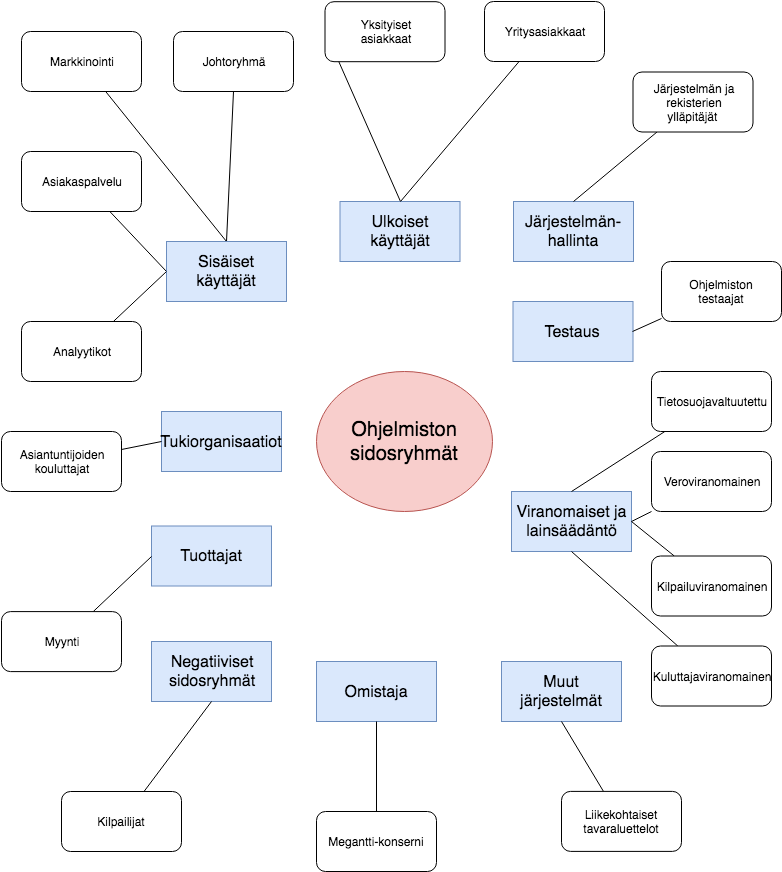
\includegraphics[width=\textwidth]{sidosryhmat.png}
		\caption{Ohjelmiston sidosryhmät} % Raportissa tulee olla selite jokaisen kuvan/kuvion/taulukon alla
		\label{img:sidosryhmat}
	\end{figure}

	Taulukkoon \ref{tab:sidosryhmataulukko} on kerätty tietoja sidosrymistä ja niiden suhteista.

\section{Alustavat havaitut vaatimukset ja luokittelu}
Taulukossa \ref{tab:sidosryhmataulukko} on havainnollistettu alustavia vaatimuksia. Taulukossa on myös määritelty vaatimusten keskinäisiä tärkeysjärjestyksiä.

    
\section{Vaatimusten keruuprojektin aikataulu}

	Vaatimusten keruun aikatulua on havainnollistettu Gantt-taulukon muodossa (Liitteessä \ref{aikatauluesimerkki}). Taulukosta ilmenee mikä vaatimusten keruumenetelmä on käytössä milloinkin.


    %\chapter{Vaatimukset ja järjestelmän kuvaus} % Itse luvun otsikko. Huom ei numeroa!                                         santeri on ruma
\label{kuvaus} % Tähän kappaleeseen voi viitata \ref{kuvaus}
\thispagestyle{fancy} % Tarvitaan, jotta header/footer näkyvät otsikkosivuilla


\section{Mallintaminen}  % 3.1
    Tässä kappaleessa kuvaillaan kaksi käyttäjätarinaa. 


\subsection{Kayttotapauskaavio(t)}    % 3.1.1

\subsubsection{Käyttäjätapaus 1: Käyttäjätietojen tarkastelu}   % 3.1.1.1

    Antti Asiakas haluaa tarkastella itseään koskevia tietoja sekä raportteja. Antin tulee valita etusivulta löytyvä
    \textit{Omat tiedot} -painike, jotta hän pääsee katsomaan omia tietojaan. 

    Täältä Antti voi:

    \begin{itemize}
        \item tarkastella ja muuttaa omia yhteystietojaan
        \item tarkastella itseään koskevia raportteja
        \item poistaa itsensä järjestelmästä
        \item kirjautua ulos
    \end{itemize}

    Jos Antti valitsee itseään koskevat raportit, järjestelmä esittää hänelle hänen oman ostohistoriansa,
    voimassa olevat alennukset sekä mahdolliset suurostobonukset.
    Jos Antilla ei ole aiempaa historiaa Megantin kanssa, järjestelmä ei tarjoa hänelle raporttia.

\subsubsection{Käyttäjätapaus 2: Personoidun tarjouksen\/tajouksien luonti ja lähettäminen}     % 3.1.1.2

    Järjestelmä ehdottaa Mikko Myyntitykille mahdollista alennusta koskien tiettyä asiakasryhmää.
    Mahdollinen alennus perustuu järjestelmän omiin sisäisiin statistiikkoihin ja algoritmeihin.
    Mikko voi hyväksyä, olla hyväksymättä alennusta, tai halutessaan määritellä tarjouksen itse.
    Jos Mikko syöttää järjestelmään alennuksen, joka on erittäin suuri, järjestelmä antaa hänelle varoituksen.
    Mikko voi myös tarkastaa, että järjestelmä ei luo alennuksia, jotka ovat liian suuria tai pieniä.
    Alennusta myönnettäessä määritellään sen suuruus, kesto, tuoteryhmät sekä asiakaskohderyhmä.

    Jos jonkinlainen alennus myönnetään, järjestelmä lähettää asiakasryhmälle sähköisen ilmoituksen alennuksesta (tarjouskirje).

\subsection{Tietoyhteyskaavio(t)}   % 3.1.2


\subsection{Navigointikaavio}     % 3.1.3


\section{Käyttöliittymä}  % 3.2
    % Rautalankamallit neljästäkäyttöliittymänäkymästä (view) ja esimerkki mahdollisista ikkunoista (dialog). 
    % Pitää olla vähintään yleisnäkymä/päänäyttö, asiakkaan tietoihin liittyvä näkymä ja raportteihin liittyvä näkymä



\section{Vaatimukset}       % 3.3
    % Vaatimusten keruun perusteella täydennetty taulukko (alkuperäiset kehyskertomuksen mukaiset ja vaatimuksen keruussa löydetyt uudet) vaatimuksista, joko suoraan dokumenttiin tai liitteenä

    \subsection{Esimerkkivaatimus 1}
        % Tarkempi kuvaus toiminnallisesta vaatimuksesta, joka ei ole suoraan sidoksissa käyttäjän tekemisiin (esim joku automaattitoiminnoista)

    \subsection{Esimerkkivaatimus 2}
        % Tarkempi kuvaus ei-toiminnallisesta vaatimuksesta


    % Esimerkkivaatimuksen perusteella lukijan tulisi ymmärtää, mitä vaatimuksen perusteella 
    % järjestelmässä tapahtuu/mitä järjestelmä tekeeeli miten järjestelmän toiminta näkyy käyttäjille. 
    % Ei tarvitsemennä teknisiin ratkaisuihin (tietokantahaut jne)



\section{Ympäristö}     % 3.4
    \subsection{Liittyvät järjestelmät}     % 3.4.1
        % Mitä liittyviä järjestelmiä on (esim vanha järjestelmä, viranomaisjärjestelmät, muut yrityksen järjestelmät)? Mitä vaatimuksia ne asettavat määrittelydokumentin järjestelmälle?


    \subsection{Tarvittavat yhteydet ja muut ympäristön vaatimukset}  % 3.4.2
        % Ympäristön (toiminta-tai käyttöympäristö) asettamia vaatimuksia? Mitä vaaditaan järjestelmältä, mitä järjestelmä vaatii ympäristöltä.


\section{Jatkokehitysajatukset}     % 3.5

    Vaikka järjestelmä on tarkoitettu nykyisellä rakenteella Megantti konsernin käyttöön, niin sitä on kuitenkin tulevaisuudessa
    mahdollisuus jatkokehittää ja tuotteistaa, jolloin Megantti voisi tarjota sitä muille yrityksille valmiina CRM:änä.

    Myös, jos Megantti laajentaa toimintaa kansainvälisille markkinoille ja näille tytäryhtiöille otetaan myös käyttöön rakennettava
    CMR, tulee vähintään järjestelmän kieliä lisätä. Todennäköisesti myös uusia rajapintajärjestelmiä tulisi ottaa huomioon ja implementoida.


\section{Avoimet asiat}     % 3.6
    % Avoimeksi jääneitä asioita esim. määrittelyn aikataulun kiireen tai jonkin muun syyn takia.



   


    \printglossaries

    % LIITTEET
    \appendix

    \chapter{Aikatauluesimerkki}
\begin{landscape}
\begin{figure}
	\begin{ganttchart}{1}{28}[
	    x unit  = 3.3cm	
		]
    % TODO Tästä saa vielä hienon kun vöhön käyttää aikaa hiomiseen. Atm karkea perusmalli
    \gantttitle{Neljän viikon aikajakso}{28} \\
    \gantttitlelist{1,...,28}{1} \\
    
\ganttgroup{Epäsuorat metodit}{1}{13} \\
	\ganttbar{Taustatutkimus}{1}{10} \\
	\ganttbar{Kyselyt}{3}{10} \\
	\ganttbar{Prototyyppi 1}{10}{13} \\
	\ganttmilestone{Prototyyppi 1 valmis}{14} \\

\ganttgroup{Suorat metodit}{15}{28} \\
	\ganttbar{Haastattelut}{15}{22} \\
	\ganttbar{Ryhmätapaaminen}{15}{22} \\
	\ganttbar{Prototyyppi 2}{20}{28} \\
	\ganttbar{Havainnointi}{3}{18} \\

	% linkit / nuolet

	% epäsuorat
	\ganttlink{elem1}{elem4} \\
	\ganttlink{elem2}{elem4} \\
	\ganttlink{elem3}{elem4} \\
	
	% Suorat metodit osa
	\ganttlink{elem6}{elem8} \\
	\ganttlink{elem7}{elem8} \\

\end{ganttchart}

\caption{Ehdotus eri menetelmien aikataulutuksesta Gantt\-kaavion muodossa}
\label{aikatauluesimerkki}
\end{figure}
\end{landscape}

    \chapter{Taulukko keskeisistä vaatimuksista}

\begin{landscape}
\begin{table}[]
\resizebox{21cm}{!}{% use resizebox with textwidth
    \begin{tabular}{llll}
    \multicolumn{4}{l}{Prioriteeti (1=Vähiten tärkeä, 2= Jonkin verran tärkeä, 3= Erittäin tärkeä)  Luokat (T=Tuottajat, H=Hyödyntäjät, J=Järjestelmävaatimus)}                                                                                                                                                                           \\ \hline
    \multicolumn{1}{|l|}{{\color[HTML]{000000} \textbf{Prioriteetti}}} & \multicolumn{1}{l|}{{\color[HTML]{000000} \textbf{Lähde}}} & \multicolumn{1}{l|}{{\color[HTML]{000000} \textbf{Luokka}}} & \multicolumn{1}{l|}{{\color[HTML]{000000} \textbf{Vaatimus}}}                                                \\ \hline
    \multicolumn{1}{|l|}{3}                                            & \multicolumn{1}{l|}{Haastattelut}                                      & \multicolumn{1}{l|}{T/H}                                    & \multicolumn{1}{l|}{Asiakastietojärjestelmää tulee pystyä käyttää eri päätelaitteilta.}                       \\ \hline
    \multicolumn{1}{|l|}{3}                                            & \multicolumn{1}{l|}{Taustatutkimus}                                      & \multicolumn{1}{l|}{J}                                    & \multicolumn{1}{l|}{Järjestelmän tulee noudattaa GDPR:ää.}                                                   \\ \hline
    \multicolumn{1}{|l|}{3}                                            & \multicolumn{1}{l|}{Taustatutkimus}                                      & \multicolumn{1}{l|}{J}                                      & \multicolumn{1}{l|}{Järjestelmän tulee olla yhteensopiva muiden olemassa olevien järjestelmien kanssa.}      \\ \hline
    \multicolumn{1}{|l|}{2}                                            & \multicolumn{1}{l|}{Havainnointi}                                      & \multicolumn{1}{l|}{T}                                      & \multicolumn{1}{l|}{Asiakkaiden tiedot tulee pystyä etsiä järjestelmästä nopeasti.}                           \\ \hline
    \multicolumn{1}{|l|}{3}                                            & \multicolumn{1}{l|}{Taustatutkimus}                                      & \multicolumn{1}{l|}{J}                                      & \multicolumn{1}{l|}{Järjestelmä rakennetaan olemassa olevan olevan ERP SQL constructoreiden päälle.}          \\ \hline
    \multicolumn{1}{|l|}{2}                                            & \multicolumn{1}{l|}{Prototyypit}                                      & \multicolumn{1}{l|}{T}                                      & \multicolumn{1}{l|}{Järjestelmän tulee seurata asiakkaiden ostoskäyttäytymistä.}                              \\ \hline
    \multicolumn{1}{|l|}{3}                                            & \multicolumn{1}{l|}{Havainnointi}                                      & \multicolumn{1}{l|}{T}                                      & \multicolumn{1}{l|}{Järjestelmän tulee pitää lokia kaikista tapahtumista.}                                   \\ \hline
    \multicolumn{1}{|l|}{2}                                            & \multicolumn{1}{l|}{Taustatutkimus}                                      & \multicolumn{1}{l|}{T}                                      & \multicolumn{1}{l|}{Järjestelmän pitää pystyä analysoida ja profiloida asiakkaita.}                         \\ \hline
    \multicolumn{1}{|l|}{1}                                            & \multicolumn{1}{l|}{Prototyypit/Haastattelut}                                      & \multicolumn{1}{l|}{T/H}                                    & \multicolumn{1}{l|}{Järjestelmän tulee olla helppokäyttöinen(Graphical user Interface.)}                    \\ \hline
    \multicolumn{1}{|l|}{1}                                            & \multicolumn{1}{l|}{Prototyypit}                                      & \multicolumn{1}{l|}{J}                                    & \multicolumn{1}{l|}{Järjestelmässä tulee olla monipuolisia toimintoja, kuten ostoshistoria, selainhistoria.}\\ \hline
    \multicolumn{1}{|l|}{2}                                            & \multicolumn{1}{l|}{Haastattelut}                                      & \multicolumn{1}{l|}{J}                                    & \multicolumn{1}{l|}{Järjestelmän luotettavuus tulee taata.}                                                 \\ \hline
    \multicolumn{1}{|l|}{1}                                            & \multicolumn{1}{l|}{Ryhmätapaamiset}                                      & \multicolumn{1}{l|}{H}                                    & \multicolumn{1}{l|}{Järjestelmän tulee pystyä yksilöllistää asiakkaan markkinointia.}                       \\ \hline
    \multicolumn{1}{|l|}{2}                                            & \multicolumn{1}{l|}{Ryhmätapaamiset}                                      & \multicolumn{1}{l|}{T}                                    & \multicolumn{1}{l|}{Järjestelmän tulee pitää kirjaa järjestelmätapahtumista.}                               \\ \hline
    \multicolumn{1}{|l|}{3}                                            & \multicolumn{1}{l|}{Taustatutkimus}                                      & \multicolumn{1}{l|}{J}                                    & \multicolumn{1}{l|}{Järjestelmän backendin tulee olla erotettu frontendistä (headless)}                               \\ \hline
    \multicolumn{1}{|l|}{3}                                            & \multicolumn{1}{l|}{Taustatutkimus}                                      & \multicolumn{1}{l|}{J}                                    & \multicolumn{1}{l|}{Järjestelmällä tulee olla web pohjainen skaalautuva käyttöliittymä}                               \\ \hline
   

    \end{tabular}
}
    \caption{Taulukko keskeisistä vaatimuksista}
    \label{tab:vaatimukset}
    \end{table}	
\end{landscape}

    \chapter{Sidosryhmätaulukko}

% Please add the following required packages to your document preamble:
% \usepackage[table,xcdraw]{xcolor}
% If you use beamer only pass "xcolor=table" option, i.e. \documentclass[xcolor=table]{beamer}
\begin{landscape}
\begin{table}[]
\label{tab:sidosryhmataulukko}
\resizebox{21cm}{!}{% use resizebox with textwidth
\begin{tabular}{llllllllllllllll}
Sidosryhmäanalyysin tulokset                                                                                                                       & V1.0                                                                                                                &                                                                                                                  &                                                                                                &                                                                                    &                                  &                                   &                                        &                                                                                         &                                      &                                                       &                                      &                                                                                                    &                                     &                                   &                                 \\
                                                                                                                                                   &                                                                                                                     &                                                                                                                  &                                                                                                &                                                                                    &                                  &                                   &                                        &                                                                                         &                                      &                                                       &                                      &                                                                                                    &                                     &                                   &                                 \\
\rowcolor[HTML]{9B9B9B} 
{\color[HTML]{CB0000} \begin{tabular}[c]{@{}l@{}}Sidosryhmäluokka\\   (laajempi sidosryhmäluokka, esim. käyttäjä tai\\   hyödyntäjä)\end{tabular}} & {\color[HTML]{CB0000} \begin{tabular}[c]{@{}l@{}}Sidosryhmä (esim. IT-osasto,\\   markkinointiosasto)\end{tabular}} & {\color[HTML]{CB0000} \begin{tabular}[c]{@{}l@{}}Sidosryhmän oikeutus (Miksi se on\\   osallinen?)\end{tabular}} & {\color[HTML]{3531FF} \begin{tabular}[c]{@{}l@{}}Tarpeellinen\\   osallistuminen\end{tabular}} & {\color[HTML]{3531FF} Tiedonkeruumenetelmä}                                        & {\color[HTML]{3531FF} Rajapinta} & {\color[HTML]{3531FF} Tavoitteet} & {\color[HTML]{3531FF} Toiminnallisuus} & {\color[HTML]{3531FF} \begin{tabular}[c]{@{}l@{}}Tekniset\\   rajoitukset\end{tabular}} & {\color[HTML]{3531FF} Käyttökokemus} & {\color[HTML]{3531FF} Käytettävyys  (cross platform)} & {\color[HTML]{3531FF} Siirrettävyys} & {\color[HTML]{3531FF} \begin{tabular}[c]{@{}l@{}}Liiketoiminnalliset\\   rajoitukset\end{tabular}} & {\color[HTML]{3531FF} Suorituskyky} & {\color[HTML]{3531FF} Tietoturva} & {\color[HTML]{3531FF} Ylläpito} \\
                                                                                                                                                   &                                                                                                                     &                                                                                                                  &                                                                                                &                                                                                    &                                  &                                   &                                        &                                                                                         &                                      &                                                       &                                      &                                                                                                    &                                     &                                   &                                 \\
\begin{tabular}[c]{@{}l@{}}Operatiivinen\\   toiminta\end{tabular}                                                                                 &                                                                                                                     &                                                                                                                  &                                                                                                &                                                                                    &                                  &                                   &                                        &                                                                                         &                                      &                                                       &                                      &                                                                                                    &                                     &                                   & x                               \\
\begin{tabular}[c]{@{}l@{}}Rekisterien\\   ylläpito\end{tabular}                                                                                   & IT-osasto                                                                                                           & Sisällönhaltija                                                                                                  & \begin{tabular}[c]{@{}l@{}}Määrittely \&\\   käyttöönotto\end{tabular}                         & \begin{tabular}[c]{@{}l@{}}haastattelut,\\   ryhmätapaamiset, protot\end{tabular}  &                                  &                                   & x                                      &                                                                                         &                                      &                                                       &                                      &                                                                                                    &                                     &                                   & x                               \\
\begin{tabular}[c]{@{}l@{}}Järjestelmän\\   hallinta\end{tabular}                                                                                  & IT-osasto                                                                                                           & Pääkäyttäjä                                                                                                      & \begin{tabular}[c]{@{}l@{}}Määrittely \&\\   käyttöönotto\end{tabular}                         & \begin{tabular}[c]{@{}l@{}}haastattelut,\\   ryhmätapaamiset, protot\end{tabular}  &                                  &                                   & x                                      & x                                                                                       &                                      &                                                       &                                      &                                                                                                    &                                     &                                   &                                 \\
                                                                                                                                                   &                                                                                                                     &                                                                                                                  &                                                                                                &                                                                                    &                                  &                                   &                                        &                                                                                         &                                      &                                                       &                                      &                                                                                                    &                                     &                                   &                                 \\
\begin{tabular}[c]{@{}l@{}}Pääasialliset\\   käyttäjät\end{tabular}                                                                                &                                                                                                                     &                                                                                                                  &                                                                                                &                                                                                    &                                  &                                   &                                        &                                                                                         &                                      &                                                       &                                      &                                                                                                    &                                     &                                   &                                 \\
\begin{tabular}[c]{@{}l@{}}Käyttäjä /\\   hyödyntäjä\end{tabular}                                                                                  & Markkinointiosasto                                                                                                  & Päähyödyntäjä                                                                                                    & Määrittely                                                                                     & \begin{tabular}[c]{@{}l@{}}ryhmätapaamiset,\\   havainnointi, protot\end{tabular}  &                                  &                                   & x                                      &                                                                                         & x                                    & x                                                     &                                      &                                                                                                    &                                     &                                   &                                 \\
\begin{tabular}[c]{@{}l@{}}Käyttäjä /\\   hyödyntäjä\end{tabular}                                                                                  & Myyntiosasto                                                                                                        & Päähyödyntäjä                                                                                                    & Määrittely                                                                                     & \begin{tabular}[c]{@{}l@{}}ryhmätapaamiset,\\   havainnointi, protot\end{tabular}  &                                  &                                   & x                                      &                                                                                         & x                                    & x                                                     &                                      &                                                                                                    &                                     &                                   &                                 \\
Hyödyntäjä                                                                                                                                         & Analyytikot                                                                                                         & Hyödyntäjä                                                                                                       & Määrittely                                                                                     & haastattelut, kyselyt                                                              &                                  &                                   & x                                      &                                                                                         &                                      &                                                       &                                      &                                                                                                    &                                     &                                   &                                 \\
\begin{tabular}[c]{@{}l@{}}Käyttäjä /\\   hyödyntäjä\end{tabular}                                                                                  & Asiakaspalvelu                                                                                                      & Hyödyntäjä                                                                                                       & Määrittely                                                                                     & haastattelut, kyselyt                                                              &                                  &                                   &                                        &                                                                                         & x                                    &                                                       &                                      &                                                                                                    &                                     &                                   &                                 \\
                                                                                                                                                   &                                                                                                                     &                                                                                                                  &                                                                                                &                                                                                    &                                  &                                   &                                        &                                                                                         &                                      &                                                       &                                      &                                                                                                    &                                     &                                   &                                 \\
\begin{tabular}[c]{@{}l@{}}Ulkoiset\\   käyttäjät\end{tabular}                                                                                     &                                                                                                                     &                                                                                                                  &                                                                                                &                                                                                    &                                  &                                   &                                        &                                                                                         &                                      &                                                       &                                      &                                                                                                    &                                     &                                   &                                 \\
Hyödyntäjä                                                                                                                                         & Henkilöasiakas                                                                                                      & Mahdollinen käyttäjä                                                                                             & Määrittely                                                                                     & taustatutkimus                                                                     &                                  &                                   &                                        &                                                                                         &                                      & x                                                     &                                      & x                                                                                                  &                                     &                                   &                                 \\
Hyödyntäjä                                                                                                                                         & Yritykset                                                                                                           & Mahdollinen käyttäjä                                                                                             & Määrittely                                                                                     & taustatutkimus                                                                     &                                  &                                   &                                        &                                                                                         &                                      & x                                                     &                                      & x                                                                                                  &                                     &                                   &                                 \\
                                                                                                                                                   &                                                                                                                     &                                                                                                                  &                                                                                                &                                                                                    &                                  &                                   &                                        &                                                                                         &                                      &                                                       &                                      &                                                                                                    &                                     &                                   &                                 \\
\begin{tabular}[c]{@{}l@{}}Ympäristön\\   tahot\end{tabular}                                                                                       &                                                                                                                     &                                                                                                                  &                                                                                                &                                                                                    &                                  &                                   &                                        &                                                                                         &                                      &                                                       &                                      &                                                                                                    &                                     &                                   &                                 \\
\begin{tabular}[c]{@{}l@{}}Muut\\   järjestelmät\end{tabular}                                                                                      & Muut järjestelmät                                                                                                   & Rajapinta                                                                                                        & Koko projekti                                                                                  & \begin{tabular}[c]{@{}l@{}}taustatutkimus,\\   protot\end{tabular}                 & x                                &                                   & x                                      & x                                                                                       &                                      & x                                                     & x                                    &                                                                                                    &                                     & x                                 &                                 \\
\begin{tabular}[c]{@{}l@{}}Muut tahot /\\   vaikuttaja\end{tabular}                                                                                & \begin{tabular}[c]{@{}l@{}}Tietosuojavaltuuttettu\\   (GDPR)\end{tabular}                                           & Vaikuttaja                                                                                                       & Määrittely                                                                                     & taustatutkimus                                                                     &                                  &                                   &                                        & x                                                                                       &                                      &                                                       &                                      & x                                                                                                  &                                     & x                                 &                                 \\
\begin{tabular}[c]{@{}l@{}}Muut tahot /\\   vaikuttaja\end{tabular}                                                                                & Kilpailuviranomainen                                                                                                & Vaikuttaja                                                                                                       & Määrittely                                                                                     & taustatutkimus                                                                     &                                  &                                   &                                        &                                                                                         &                                      &                                                       &                                      & x                                                                                                  &                                     &                                   &                                 \\
\begin{tabular}[c]{@{}l@{}}Muut tahot /\\   vaikuttaja\end{tabular}                                                                                & Veroviranomainen                                                                                                    & Vaikuttaja                                                                                                       & Määrittely                                                                                     & taustatutkimus                                                                     &                                  &                                   &                                        &                                                                                         &                                      &                                                       &                                      & x                                                                                                  &                                     &                                   &                                 \\
\begin{tabular}[c]{@{}l@{}}Muut tahot /\\   vaikuttaja\end{tabular}                                                                                & Kuluttajaviranomainen                                                                                               & Vaikuttaja                                                                                                       & Määrittely                                                                                     & taustatutkimus                                                                     &                                  &                                   &                                        &                                                                                         &                                      &                                                       &                                      & x                                                                                                  &                                     &                                   &                                 \\
Vaikuttaja                                                                                                                                         & Rahoittaja                                                                                                          & Vaikuttaja                                                                                                       & Koko projekti                                                                                  & \begin{tabular}[c]{@{}l@{}}ryhmätapaamiset,\\   protot\end{tabular}                &                                  & x                                 &                                        &                                                                                         &                                      &                                                       &                                      &                                                                                                    &                                     &                                   &                                 \\
Hyödyntäjä                                                                                                                                         & Varastotoimijat                                                                                                     & \begin{tabular}[c]{@{}l@{}}Hyödyntäjä /\\   rajapinta\end{tabular}                                               & Määrittely                                                                                     & taustatutkimus                                                                     & x                                &                                   &                                        &                                                                                         &                                      &                                                       &                                      &                                                                                                    &                                     &                                   &                                 \\
\begin{tabular}[c]{@{}l@{}}Hyödyntäjä /\\   alihankkija\end{tabular}                                                                               & Logistiikka                                                                                                         & Rajapinta                                                                                                        & Määrittely                                                                                     & taustatutkimus                                                                     & x                                &                                   & x                                      &                                                                                         &                                      &                                                       & x                                    &                                                                                                    &                                     &                                   &                                 \\
                                                                                                                                                   &                                                                                                                     &                                                                                                                  &                                                                                                &                                                                                    &                                  &                                   &                                        &                                                                                         &                                      &                                                       &                                      &                                                                                                    &                                     &                                   &                                 \\
Ydinprojektiryhmä                                                                                                                                  &                                                                                                                     &                                                                                                                  &                                                                                                &                                                                                    &                                  &                                   &                                        &                                                                                         &                                      &                                                       &                                      &                                                                                                    &                                     &                                   &                                 \\
Omistaja                                                                                                                                           & Megantti                                                                                                            & Omistaja                                                                                                         & \begin{tabular}[c]{@{}l@{}}Määrittely \&\\   käyttöönotto\end{tabular}                         & \begin{tabular}[c]{@{}l@{}}ryhmätapaamiset,\\   kyselyt\end{tabular}               &                                  & x                                 &                                        &                                                                                         &                                      &                                                       &                                      &                                                                                                    &                                     &                                   &                                 \\
\begin{tabular}[c]{@{}l@{}}Toimeksiantaja\\   / hyödyntäjä\end{tabular}                                                                            & Johtoryhmä                                                                                                          & Omistaja / hyödyntäjä                                                                                            & \begin{tabular}[c]{@{}l@{}}Määrittely \&\\   käyttöönotto\end{tabular}                         & \begin{tabular}[c]{@{}l@{}}ryhmätapaamiset,\\   kyselyt, havainnointi\end{tabular} &                                  & x                                 & x                                      &                                                                                         &                                      &                                                       &                                      &                                                                                                    &                                     &                                   &                                 \\
Muut tahot                                                                                                                                         & Projektipäällikkö                                                                                                   & Toteuttaja                                                                                                       & Koko projekti                                                                                  &                                                                                    &                                  & x                                 &                                        & x                                                                                       &                                      &                                                       &                                      &                                                                                                    & x                                   &                                   &                                 \\
                                                                                                                                                   &                                                                                                                     &                                                                                                                  &                                                                                                &                                                                                    &                                  &                                   &                                        &                                                                                         &                                      &                                                       &                                      &                                                                                                    &                                     &                                   &                                 \\
\begin{tabular}[c]{@{}l@{}}Projektin\\   toteuttajat\end{tabular}                                                                                  &                                                                                                                     &                                                                                                                  &                                                                                                &                                                                                    &                                  &                                   &                                        &                                                                                         &                                      &                                                       &                                      &                                                                                                    &                                     &                                   &                                 \\
Tuottaja                                                                                                                                           & Ohjelmistotuottajat                                                                                                 & Toteuttaja                                                                                                       & Koko projekti                                                                                  &                                                                                    &                                  &                                   & x                                      &                                                                                         &                                      &                                                       &                                      &                                                                                                    &                                     &                                   &                                 \\
Tuottaja                                                                                                                                           & Ohjelmistotestaajat                                                                                                 & Toteuttaja                                                                                                       & Koko projekti                                                                                  &                                                                                    &                                  &                                   & x                                      &                                                                                         &                                      &                                                       &                                      &                                                                                                    &                                     &                                   &                                 \\
                                                                                                                                                   &                                                                                                                     &                                                                                                                  &                                                                                                &                                                                                    &                                  &                                   &                                        &                                                                                         &                                      &                                                       &                                      &                                                                                                    &                                     &                                   &                                 \\
Kilpailijat                                                                                                                                        & \begin{tabular}[c]{@{}l@{}}esim. Gigantti ja\\   Verkkokauppa.com\end{tabular}                                      & kilpailija                                                                                                       & Määrittely                                                                                     & taustatutkimus                                                                     &                                  &                                   &                                        &                                                                                         &                                      &                                                       &                                      & x                                                                                                  &                                     &                                   &                                 \\
                                                                                                                                                   &                                                                                                                     &                                                                                                                  &                                                                                                &                                                                                    &                                  &                                   &                                        &                                                                                         &                                      &                                                       &                                      &                                                                                                    &                                     &                                   &                                 \\
                                                                                                                                                   &                                                                                                                     &                                                                                                                  &                                                                                                &                                                                                    &                                  &                                   &                                        &                                                                                         &                                      &                                                       &                                      &                                                                                                    &                                     &                                   &                                
\end{tabular}
}
\end{table}
\end{landscape}



\end{document}
